 \documentclass[11pt]{article} 
\usepackage[english]{babel}
\usepackage[utf8]{inputenc}
\usepackage[margin=0.5in]{geometry}
\usepackage{amsmath}
\usepackage{amsthm}
\usepackage{amsfonts}
\usepackage{amssymb}
\usepackage[usenames,dvipsnames]{xcolor}
\usepackage{graphicx}
\usepackage[siunitx]{circuitikz}
\usepackage{tikz}
\usepackage{tkz-berge}
\usetikzlibrary{positioning, automata, backgrounds}
\usepackage[colorinlistoftodos, color=orange!50]{todonotes}
\usepackage{hyperref}
\usepackage[numbers, square]{natbib}
\usepackage{fancybox}
\usepackage{epsfig}
\usepackage{soul}
\usepackage[framemethod=tikz]{mdframed}
\usepackage[shortlabels]{enumitem}
\usepackage[version=4]{mhchem}
\usepackage{multicol}
\usepackage{forest}
\usepackage{mathtools}
\usepackage{comment}
\usepackage{enumitem}
\usepackage[utf8]{inputenc}
\usepackage{listings}
\usepackage{color}
\usepackage[numbers]{natbib}
\usepackage{subfiles}
\usepackage{tkz-berge}
\usepackage{algorithm}
\usepackage[noend]{algpseudocode}


\newtheorem{prop}{Proposition}[section]
\newtheorem{thm}{Theorem}[section]
\newtheorem{lemma}{Lemma}[section]
\newtheorem{cor}{Corollary}[prop]

\theoremstyle{definition}
\newtheorem{definition}{Definition}

\theoremstyle{definition}
\newtheorem{required}{Problem}

\theoremstyle{definition}
\newtheorem{ex}{Example}

\newcommand{\interval}[4]{\draw (#2, #1) -- (#3, #1); % Usage: \interval{height}{start}{end}{label}
\draw (#2, #1-0.11) -- (#2, #1+0.11); % draw left whisker
\draw (#3, #1-0.11) -- (#3, #1+0.11); % draw right whisker
\node[] at (#2-0.25, #1) {#4};
}


\setlength{\marginparwidth}{3.4cm}
%#########################################################

%To use symbols for footnotes
\renewcommand*{\thefootnote}{\fnsymbol{footnote}}
%To change footnotes back to numbers uncomment the following line
%\renewcommand*{\thefootnote}{\arabic{footnote}}

% Enable this command to adjust line spacing for inline math equations.
% \everymath{\displaystyle}

% _______ _____ _______ _      ______ 
%|__   __|_   _|__   __| |    |  ____|
%   | |    | |    | |  | |    | |__   
%   | |    | |    | |  | |    |  __|  
%   | |   _| |_   | |  | |____| |____ 
%   |_|  |_____|  |_|  |______|______|
%%%%%%%%%%%%%%%%%%%%%%%%%%%%%%%%%%%%%%%

\title{
\normalfont \normalsize 
\textsc{CSCI 3104 Fall 2021 \\ 
Instructors: Profs. Chen and Layer} \\
[10pt] 
\rule{\linewidth}{0.5pt} \\[6pt] 
\huge Problem Set 10 \\
\rule{\linewidth}{2pt}  \\[10pt]
}
%\author{Your Name}
\date{}

\begin{document}
\definecolor {processblue}{cmyk}{0.96,0,0,0}
\maketitle


%%%%%%%%%%%%%%%%%%%%%%%%%
%%%%%%%%%%%%%%%%%%%%%%%%%%
%%%%%%%%%%FILL IN YOUR NAME%%%%%%%
%%%%%%%%%%AND STUDENT ID%%%%%%%%
%%%%%%%%%%%%%%%%%%%%%%%%%%
\noindent
Due Date \dotfill April 26 \\
Name \dotfill \textbf{Chengming Li} \\
Student ID \dotfill \textbf{109251991} \\
Collaborators \dotfill \textbf{List Your Collaborators Here}

\tableofcontents

\section{Instructions}
 \begin{itemize}
	\item The solutions \textbf{must be typed}, using proper mathematical notation. We cannot accept hand-written solutions. \href{http://ece.uprm.edu/~caceros/latex/introduction.pdf}{Here's a short intro to \LaTeX.}
	\item You should submit your work through the \textbf{class Canvas page} only. Please submit one PDF file, compiled using this \LaTeX \ template.
	\item You may not need a full page for your solutions; pagebreaks are there to help Gradescope automatically find where each problem is. Even if you do not attempt every problem, please submit this document with no fewer pages than the blank template (or Gradescope has issues with it).

	\item You are welcome and encouraged to collaborate with your classmates, as well as consult outside resources. You must \textbf{cite your sources in this document.} \textbf{Copying from any source is an Honor Code violation. Furthermore, all submissions must be in your own words and reflect your understanding of the material.} If there is any confusion about this policy, it is your responsibility to clarify before the due date. 

	\item Posting to \textbf{any} service including, but not limited to Chegg, Reddit, StackExchange, etc., for help on an assignment is a violation of the Honor Code.
\end{itemize}


\newpage
\section{Standard 26 - Showing problems belong to $\textsf{P}$}
\begin{required} \label{InP}
Consider the Shortest Path problem that takes as input a graph $G=(V,E)$
and two vertices $v,t\in V$ and returns the shortest path from $v$ to $t$.
The shortest path decision problem takes as input a graph $G=(V,E)$, two a
vertices $v,t\in V$, and a value $k$, and returns True if there is a path from
$v$ to $t$ that is at most $k$ edges and False otherwise. Show that the
shortest path decision problem is in $\textsf{P}$. You are welcome and
encouraged to cite algorithms we have previously covered in class, including
known facts about their runtime.  [\textbf{Note:} To gauge the level of
detail, we expect your solutions to this problem will be 2-4 sentences. We are
not asking you to analyze an algorithm in great detail.]

\end{required}
\begin{proof}[Answer]
\begin{itemize}
\item As given in the question, the decision problem is: is there a path from $v$ to $t$ that is at most k edges.

\item We have seen Dijkstra’s algorithm computes the shortest path from $v$ to $t$ in time O($\mid V\mid + \mid E \mid log(\mid V \mid)$) with min-priority queue. And usually, the time complexity of Dijkstra's algorithm is O($V^2$)

\item Thus, we can apply Dijkstra's algorithm to G. And it will return a path that is computed in \textbf{polynomial} time. Then, we could compare the number of edges in this path to the value k. If the number of edges are less or equal to k, we could assert that there is path from $v$ to $t$ in the graph G at most k edges. So, this $\textbf{Path} \in \textbf{P}$ and Shortest Path decision problem $ \in \textbf{P}$
\end{itemize}
\end{proof}


\newpage
\section{Standard 27 - Showing problems belong to $\textsf{NP}$}
\begin{required} \label{InNP}
Consider the Simple Shortest Path decision problem that takes as input a
directed graph $G=(V,E)$, a cost function $c(e)\in \mathbb{Z}$ for $e \in E$,
and two vertices $v,t\in V$. The problem returns True if there is a simple path from
$v$ to $t$ with edge weights that sum to at most $k$, and False otherwise.
Show this problem is in $\textsf{NP}$.
\end{required}

\begin{proof}[Answer]
\begin{itemize}
\item  Simple Path is the path from one vertex to another such that no vertex is visited more than once.

\item Suppose graph G has such a simple $\textbf{path}$ between $v$ to $t$  with edge weights that sum to at most $k$. There three things we need to check: is it a valid path, is it a simple path and is it length at most k.
\end{itemize}
\begin{itemize}
\item$\textbf{Claim1: Simple Shortest Path decision problem has a valid path from $v$ to $t$ }$.
\end{itemize}
In this claim, we need to check any edges in this $\textbf{path}$ is $\in E$ A. In other words , any edges in this $\textbf{path}$ is the edge in graph G. And we need to check the there is path from $v$ to $t$. The time complexity to valid this claim is O($n^2$), where n is the number of edges in this $\textbf{path}$.
\begin{itemize}
\item$\textbf{Claim2: Simple Shortest Path decision problem has a valid Simple path}$.
\end{itemize}
In this claim2, we need to check every vertex in this path has been visited precisely once.   The time complexity to check whether each vertex is included once is O(n), where n is the number of edges in this $\textbf{path}$.\\
\\The algorithm to check the whether each vertex has been visited precisely once is: define a $\textbf{Visited}$ element for each vertex. And we mark each un-visited vertex to false at the beginning of the algorithm. Once the algorithm starts, we check each vertex in this $\textbf{path}$ if it has been visited or not. if it has been visited before, then this  $\textbf{path}$ is not a simple path. if every vertex has been only visited only once, they  $\textbf{path}$ is a simple path. The time complexity is O(k), where k is number of vertex  in the  $\textbf{path}$. 
\begin{itemize}
\item$\textbf{Claim3: Simple Shortest Path decision problem has at most k edge weight}$.
\end{itemize}
In this claim 3, we need to compare the $\textbf{path}$ edge weights to k. if the edge weights are at most k, or less and equal to k, then we can assert this path has at most k edge weights. The time complexity of comparison is O(c), where c is a constant.
\begin{itemize}
\item$\textbf{Conclusion:}$.
\end{itemize}
Hence, Simple shortest path decision problem $\in$ NP if the $\textbf{path}$ pass all three claims above in polynomial time.


\item Hence, we conclude that Simple Shortest Path decision problem $\in \textbf{NP}$.

\end{proof}

\newpage
\begin{required} 
Indiana Jones is gathering $n$ artifacts from a tomb, which is about to crumble and needs to fit them into $5$ cases. Each case can carry up to $W$ kilograms, where $W$ is fixed. Suppose the weight of artifact $i$ is the positive integer $w_{i}$. Indiana Jones needs to decide if he is able to pack all the artifacts. We formalize the \textsf{Indiana Jones} decision problem as follows.
\begin{itemize}
\item \textsf{Instance:} The weights of our $n$ items, $w_{1}, \ldots, w_{n} > 0$. 
\item \textsf{Decision:} Is there a way to place the $n$ items into different cases, such that each case is carrying weight at most $W$?
\end{itemize}

\noindent Show that $\textsf{Indiana Jones} \in \textsf{NP}.$
\end{required}

\begin{proof}[Answer]
\begin{itemize}
\item Suppose we have a way to place n items into different cases, such that each case is carrying weight at most W. 
\end{itemize}
\begin{itemize}
\item$\textbf{Claim1:Indiana Jones problem has valid way to place n items into different cases}$.
\end{itemize}

We add up all items from each case and we check if the total number of items is same as n. Second, we visit every item in each case and we check if every item has been only visited once.\\
We can assert that there is a valid way to place the n items into different cases if there are n items in total and every item has been visited precisely once.\\
The time complexity of checking n items is O(n)
\begin{itemize}
\item$\textbf{Claim2:Each case has at most W weight}$.
\end{itemize}

In this claim2, for each case, we add up the weight of every item $w_i$ and we compare the total weight to W. If the total weights in each case is at most W kilograms, we can assert each case is carrying weight at most W.\\
The time complexity of this claim is O(n), because we just do summation of all those items in each case, and there is n item.

\begin{itemize}
\item$\textbf{Conclusion:}$.
\end{itemize}
Hence, the Indiana Jones $\in$ NP because claim1 and claim 2 can be solved in polynomial time.
\end{proof}

\newpage
\section{Standard 27 - $\textsf{NP}$-compelteness: Reduction}
\begin{required} \label{S30Prob1}
A student has a decision problem $L$ which they know is in the class \textsf{NP}. This student wishes to show that L is \textsf{NP}-complete. They attempt to do so by constructing a polynomial time reduction from $L$ to \textsf{SAT}, a known \textsf{NP}-complete problem. That is, the student attempts to show that $L \leq_{p} \textsf{SAT}.$ Determine if this student’s approach is
correct and justify your answer.
\end{required}

\begin{proof}[Answer]
\begin{itemize}
\item This student's approach is $\textbf{incorrect}$.
\item Student's approach is correct if we flip the statement as $\textsf{SAT} \leq_{p} \textsf{L}.$
\item The definition of NP complete is: A problem that is $\textbf{NP - hard}$ and is a member of $\textbf{NP}$
\end{itemize}

\begin{itemize}
\item$\textbf{Claim1: L is in the class NP}$.
\end{itemize}
As given in the question statement, the decision problem L is in the class NP.
\begin{itemize}
\item$\textbf{Claim2: L is in the class NP-hard}$.
\end{itemize}
SAT problem is well-known as NP-complete problem. Thus, we know that $\textsf{NP} \leq_{p} \textsf{SAT},$ and then we could know SAT is at least as hard as any NP-problem.  Hence we reduce SAT problem to L, which reduce an NP-complete problem to a NP problem. But  , L must be NP-hard because SAT is at least as hard as any NP-problem.\\
\\So, L is in the class NP-hard class. And So L is NP-complete problem.


\begin{itemize}
\item$\textbf{From the perspective of student's approach:}$.
\end{itemize}
We only know L is in the class NP so that we couldn't find a way to reduce problem L to SAT. In other words, we don't have enough information to use reductions to reduce from a NP problem to a NP-complete problem.
\end{proof}



\newpage
\begin{required} \label{NPcomp}
Consider the Simple Shortest Path decision problem that takes as input a
directed graph $G=(V,E)$, a cost function $c(e)\in \mathbb{Z}$ for $e \in E$,
and two vertices $v,t\in V$. The problem returns True if there is a simple path from
$v$ to $t$ with edge weights that sum to at most $k$, and False otherwise.
Show this problem is $\textsf{NP}$-compelte.
\end{required}

\begin{proof}[Answer]
\textbf{We show that Simple Shortest Path decision problem is in NP, and that Simple Shortest Path decision problem is in NP-hard}
\begin{itemize}
\item$\textbf{Claim1: Simple Shortest Path decision problem is in NP, Copy and Paste from Problem2}$.


Suppose graph G has such a simple $\textbf{path}$ between $v$ to $t$  with edge weights that sum to at most $k$. There three things we need to check: is it a valid path, is it a simple path and is it length at most k.\\

\begin{itemize}
\item$\textbf{ClaimA: Simple Shortest Path decision problem has a valid path from $v$ to $t$ }$.
\end{itemize}
In this claim, we need to check any edges in this $\textbf{path}$ is $\in E$ A. In other words , any edges in this $\textbf{path}$ is the edge in graph G. And we need to check the there is path from $v$ to $t$. The time complexity to valid this claim is O($n^2$), where n is the number of edges in this $\textbf{path}$.
\begin{itemize}
\item$\textbf{ClaimB: Simple Shortest Path decision problem has a valid Simple path}$.
\end{itemize}
In this claim2, we need to check every vertex in this path has been visited precisely once.   The time complexity to check whether each vertex is included once is O(n), where n is the number of edges in this $\textbf{path}$.\\
\\The algorithm to check the whether each vertex has been visited precisely once is: define a $\textbf{Visited}$ element for each vertex. And we mark each un-visited vertex to false at the beginning of the algorithm. Once the algorithm starts, we check each vertex in this $\textbf{path}$ if it has been visited or not. if it has been visited before, then this  $\textbf{path}$ is not a simple path. if every vertex has been only visited only once, they  $\textbf{path}$ is a simple path. The time complexity is O(k), where k is number of vertex  in the  $\textbf{path}$. 
\begin{itemize}
\item$\textbf{ClaimC: Simple Shortest Path decision problem has at most k edge weight}$.
\end{itemize}
In this claim 3, we need to compare the $\textbf{path}$ edge weights to k. if the edge weights are at most k, or less and equal to k, then we can assert this path has at most k edge weights. The time complexity of comparison is O(c), where c is a constant.
\begin{itemize}
\item$\textbf{Conclusion:}$.
\end{itemize}
Hence, Simple shortest path decision problem $\in$ NP if the $\textbf{path}$ pass all three claims above in polynomial time.


 Hence, we conclude that Simple Shortest Path decision problem $\in \textbf{NP}$.
\end{itemize}
\begin{itemize}
\item$\textbf{Claim2: Simple Shortest Path decision problem is in NP-Hard}$.

We show Hamiltonian Path $\leq_P$ Simple Shortest Path.\\
First, we reduce Hamiltonian Path problem to a Simple Shortest Path problem.
\begin{center}
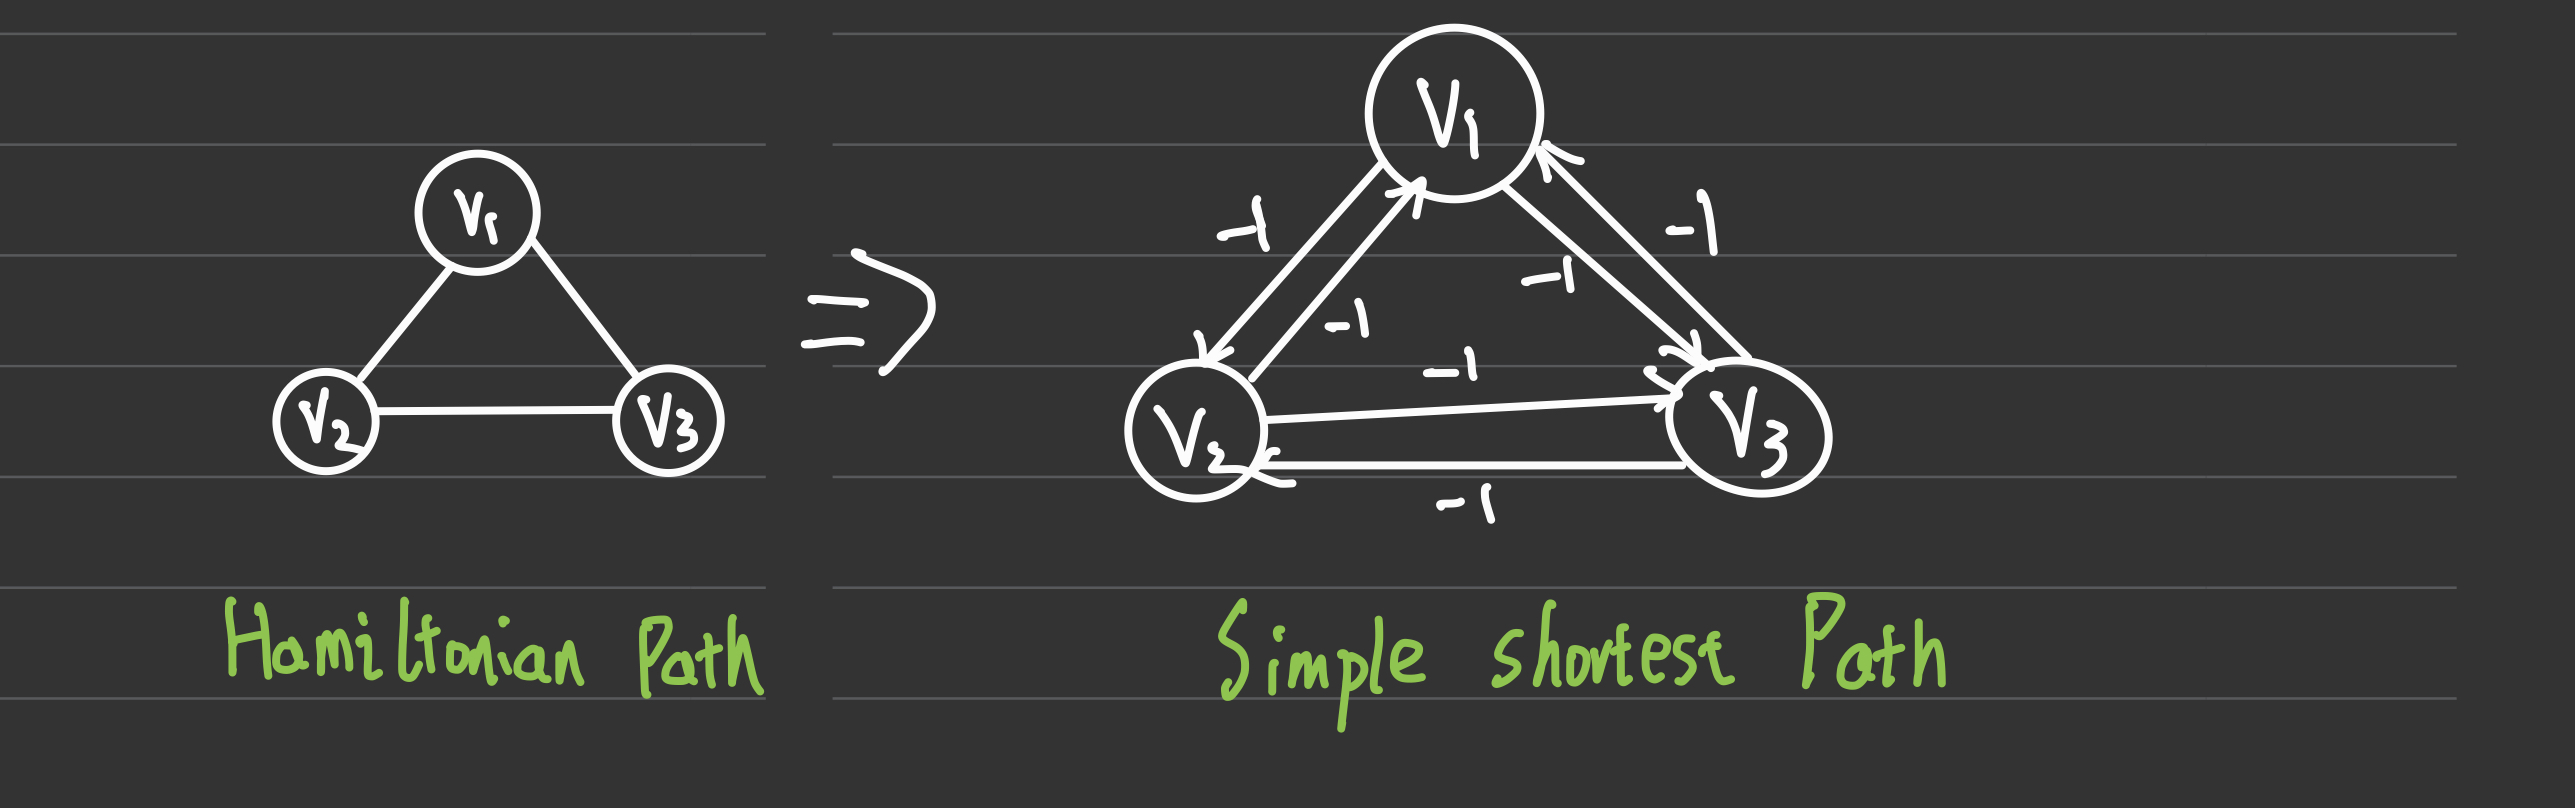
\includegraphics[width=0.7\textwidth]{IMG_0518.PNG}
\end{center}
\begin{itemize}
\item$\textbf{Construction and Reduction}$.
\end{itemize}
We replace $\{v1,v2\}$ in Hamiltonian Path to two edge $\{v1,v2\}\{v2,v1\}. $And define the cost for each new edge as -1 in simple Shortest Path. Last, replace the remaining edges in Hamiltonian Path with the same rules.\\
 The time complexity to convert the graph from Hamiltonian path to Simple Shortest Path is $\textbf{O(cV)}$, where c is constant and V is the number of vertex in graph G. 
\begin{itemize}
\item$\textbf{Examples}$.
\end{itemize}
As seen in the graph, the shortest simple path between two vertices is actually the longest simple path due to negative edge cost. 
To find Simple Shortest Path from $v$ to $t$, visiting any extra un-visited vertex will make the path shorter due to negative number. \\
For example, given v1 as v and v2 as t, the shortest path is v1 $->$ v2 $->$ v3 with cost -2. Rather than $v1->v2$ with cost -1.\\
Then, if the cost to the weighted graph is -1(V-1), where V is the number of the vertex in the graph G, we can convert the path to a path in the un-directed graph, which is a Hamiltonian path. This is because the path visits each vertex exactly once.
\begin{itemize}
\item$\textbf{Conclusion}$.
\end{itemize}
Hence, Simple Shortest Path decision problem is NP-hard since we reduce Hamiltonian Path Problem to it in Polynomial-time.
\end{itemize}
\end{proof}


\end{document} % NOTHING AFTER THIS LINE IS PART OF THE DOCUMENT



